\documentclass{article}
\title{Simple Circuit Simulator}
\date{\today}
\author{Aidan Gresko}

\usepackage{times}
\usepackage{graphicx}
\usepackage{listings}

\begin{document}
	\maketitle
	
	\section{Project Overview}
	This project implements a DC circuit simulation program for analyzing electrical networks. The program's architecture is built around multiple classes that represent fundamental circuit elements including resistors, loads, buses, and voltage sources, with extensibility for additional components as defined in the class diagram.	
	\vspace{10pt}
	
	\noindent
	The simulator is designed to solve a variety of DC circuit problems, making it valuable for both real-world electronic device development and educational applications in laboratory settings and coursework. To demonstrate the simulator's capabilities, we present an example problem focused on wire sizing based on current calculations - a common challenge in practical circuit design.	
	\newpage
	\section{Class Diagrams}
	\begin{figure}[h]
		\centering
		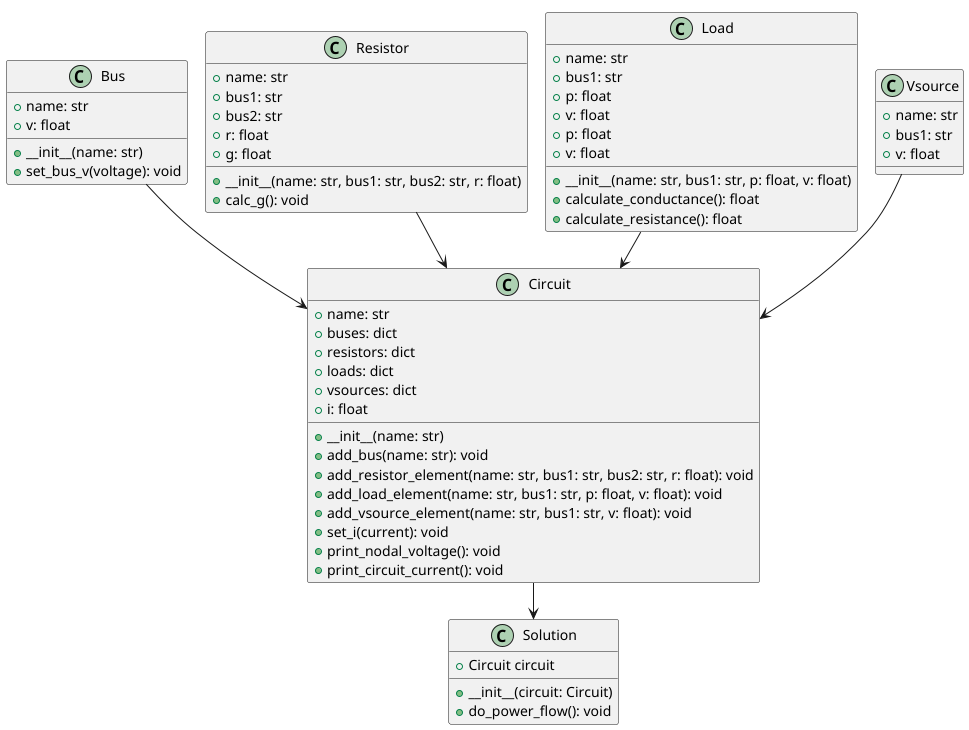
\includegraphics[scale=0.4]{/home/aidan/Desktop/Project-1---Simple-Circuit-Simulator/class_diagram.png}		
	\end{figure}
	
	\section{Relevant Equations}
	\begin{itemize}
		\item Calculate Conductance with Power and Voltage: $g = p / v^2$
		\item Calculate Resistance with voltage and power: $r = v^2 / p$
		\item Calculate Conductance with Resistance: $g = 1 / r$
		\item Calculate Current with Voltage and Resistance: $i = v / r$
		\item Calculate Voltage Drop: $voltage_drop = i * r$
		
	\end{itemize}
	
	\section{Example Case}
	
	\subsection{Problem Definition}
	Determine if a wire with 0.5$\Omega$ resistance is suitable for connecting a 1500W load (rated at 100V) to a 120V source.	
	
	\subsection{Solution Process}
	\begin{itemize}
		\item 	The simulation will calculate the load equivalent resistance: $R = V^2/P = 100^2/1500 = 6.67\Omega$
		
		\item Calculate total resistance $R_total = R_wire + R_load = 0.5 + 6.67 = 7.17 \Omega$
		
		\item Calculate circuit current: $I = V/R = 120/7.17 = 16.74A$
		
		\item Calculate voltage at load bus: $V_load = 120 - (16.74 * 0.5) = 111.63V$
	\end{itemize}
	
	The simulator works by first creating element objects (resistors, loads, buses, etc.) within the circuit class, storing them in dictionaries for easy access. The solution class then performs the calculations by accessing these dictionaries from the circuit class. The calculation process follows these steps: first, it combines the circuit's resistor resistance with the load resistance to determine total resistance. Using this total resistance, it calculates the circuit current. Finally, it sets the bus voltages by determining the voltage drop across components using the calculated current and the voltage source value.	
	
	\subsection{Expected Output}
	The setup of the circuit for completing this calculation and the code will be as follows:
	
	\begin{lstlisting}[language=Python]
from circuit import Circuit
from solution import Solution

# Circuit objects
circuit = Circuit("Wire_Test")
circuit.add_bus("Source")
circuit.add_bus("Load")
circuit.add_vsource_element("V1", "Source", 120.0)
circuit.add_resistor_element("Wire", "Source", "Load", 0.5)
circuit.add_load_element("Load1", "Load", 1500.0, 100.0)

# Solution object
solution = Solution(circuit)
solution.do_power_flow()
	\end{lstlisting}
	
	\vspace{10pt}
	
	The expected output for this circuit is to have:
	
	\vspace{10pt}
	
	\begin{tabular}{c | c }
		Bus Source Voltage & 120.000V \\
		\hline
		Bus Load Voltage & 111.628V \\
		\hline
		Current & 16.744A
	\end{tabular}
	
	\vspace{10pt}
	
	The output means that the correct gage wire to use in this scenario is a \#14 or \#12 AWG wire, but a larger one would perform a little better.
	
\end{document}
